% Neural network figures for the data-driven-I lecture notebook.
%
% Layout adapted from
%   ~/Documents/dissertation/figures/mathematical_background/neural_network.tex
% with the notation of the lecture notebooks and pyMOR colors.  The layers are
% drawn by \foreach loops rather than explicit \draw commands, so the number of
% nodes per layer is a parameter.
%
% Three variants, selected by \variant:
%   1  stationary            mu        ->  Phi_N(mu)    ~ pi_N(mu)
%   2  random-access-in-time (mu, t)   ->  Phi_N(mu,t)  ~ pi_N(mu,t)
%   3  time-vectorized       mu        ->  Phi_N(mu)    ~ [pi_N(mu,t_1), ..., pi_N(mu,t_K)]
%
% Build all three with:
%   for v in 1 2 3; do
%     pdflatex -jobname=nn_variant$v "\def\variant{$v}% Neural network figures for the data-driven-I lecture notebook.
%
% Layout adapted from
%   ~/Documents/dissertation/figures/mathematical_background/neural_network.tex
% with the notation of the lecture notebooks and pyMOR colors.  The layers are
% drawn by \foreach loops rather than explicit \draw commands, so the number of
% nodes per layer is a parameter.
%
% Three variants, selected by \variant:
%   1  stationary            mu        ->  Phi_N(mu)    ~ pi_N(mu)
%   2  random-access-in-time (mu, t)   ->  Phi_N(mu,t)  ~ pi_N(mu,t)
%   3  time-vectorized       mu        ->  Phi_N(mu)    ~ [pi_N(mu,t_1), ..., pi_N(mu,t_K)]
%
% Build all three with:
%   for v in 1 2 3; do
%     pdflatex -jobname=nn_variant$v "\def\variant{$v}% Neural network figures for the data-driven-I lecture notebook.
%
% Layout adapted from
%   ~/Documents/dissertation/figures/mathematical_background/neural_network.tex
% with the notation of the lecture notebooks and pyMOR colors.  The layers are
% drawn by \foreach loops rather than explicit \draw commands, so the number of
% nodes per layer is a parameter.
%
% Three variants, selected by \variant:
%   1  stationary            mu        ->  Phi_N(mu)    ~ pi_N(mu)
%   2  random-access-in-time (mu, t)   ->  Phi_N(mu,t)  ~ pi_N(mu,t)
%   3  time-vectorized       mu        ->  Phi_N(mu)    ~ [pi_N(mu,t_1), ..., pi_N(mu,t_K)]
%
% Build all three with:
%   for v in 1 2 3; do
%     pdflatex -jobname=nn_variant$v "\def\variant{$v}% Neural network figures for the data-driven-I lecture notebook.
%
% Layout adapted from
%   ~/Documents/dissertation/figures/mathematical_background/neural_network.tex
% with the notation of the lecture notebooks and pyMOR colors.  The layers are
% drawn by \foreach loops rather than explicit \draw commands, so the number of
% nodes per layer is a parameter.
%
% Three variants, selected by \variant:
%   1  stationary            mu        ->  Phi_N(mu)    ~ pi_N(mu)
%   2  random-access-in-time (mu, t)   ->  Phi_N(mu,t)  ~ pi_N(mu,t)
%   3  time-vectorized       mu        ->  Phi_N(mu)    ~ [pi_N(mu,t_1), ..., pi_N(mu,t_K)]
%
% Build all three with:
%   for v in 1 2 3; do
%     pdflatex -jobname=nn_variant$v "\def\variant{$v}\input{neural_networks.tex}"
%   done
%   pdftoppm -png -r 1200 nn_variant1.pdf nn_stationary   % etc., then rename
% 1200 dpi matches the other figures in this directory.

\documentclass[11pt,border=2mm]{standalone}

\usepackage{amsmath}
\usepackage{tikz}
\usetikzlibrary{positioning,calc,decorations.pathreplacing}

\definecolor{pymor_blue}{HTML}{3155a0}
\definecolor{DarkGray}{rgb}{0.274509804,0.254901961,0.235294118}

\providecommand{\variant}{1}

\tikzset{
  neuron/.style={circle, draw=pymor_blue, fill=white, minimum size=0.34cm, inner sep=0pt},
  arrow/.style={->, >=stealth, draw=DarkGray!70, line width=0.35pt, shorten >=1pt, shorten <=1pt},
  brace/.style={decorate, decoration={brace, amplitude=7pt, raise=4pt}, draw=DarkGray},
  brace mirrored/.style={decorate, decoration={brace, amplitude=7pt, mirror, raise=4pt}, draw=DarkGray},
}

\newcommand{\vsep}{0.85}   % vertical distance between neurons
\newcommand{\hsep}{1.75}   % horizontal distance between layers

% #1 layer name, #2 number of neurons, #3 x position -- vertically centred on y=0
\newcommand{\layer}[3]{%
  \foreach \i in {1,...,#2} {%
    \pgfmathsetmacro{\ypos}{-(\i - (#2+1)/2)*\vsep}%
    \node[neuron] (#1-\i) at (#3,\ypos) {};%
  }%
}

% #1 source name, #2 source count, #3 target name, #4 target count
\newcommand{\connect}[4]{%
  \foreach \i in {1,...,#2} {\foreach \j in {1,...,#4} {\draw[arrow] (#1-\i) -- (#3-\j);}}%
}

% number of input and output neurons for the selected variant
\ifnum\variant=2 \def\nin{3}\else\def\nin{2}\fi
\ifnum\variant=3 \def\nout{12}\else\def\nout{4}\fi

\begin{document}
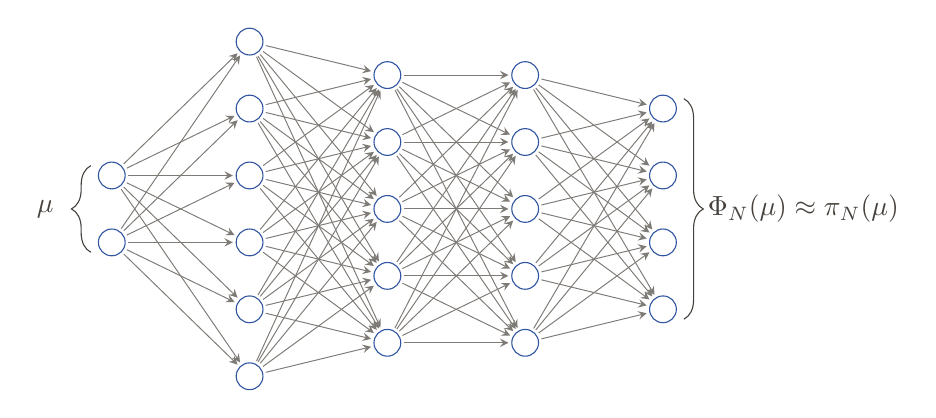
\begin{tikzpicture}

  \layer{input}{\nin}{0}
  \layer{hiddenA}{6}{\hsep}
  \layer{hiddenB}{5}{2*\hsep}
  \layer{hiddenC}{5}{3*\hsep}
  \layer{output}{\nout}{4*\hsep}

  \connect{input}{\nin}{hiddenA}{6}
  \connect{hiddenA}{6}{hiddenB}{5}
  \connect{hiddenB}{5}{hiddenC}{5}
  \connect{hiddenC}{5}{output}{\nout}

  % --- inputs --------------------------------------------------------------
  % the parameter always occupies the first two neurons; for the
  % random-access-in-time variant the time instance enters as a third input
  \draw[brace mirrored] (input-1.north west) -- (input-2.south west)
    node[midway, xshift=-0.72cm, text=DarkGray] {$\mu$};
  \ifnum\variant=2
    \node[left=0.5cm of input-3, text=DarkGray, inner sep=1pt] (t) {$t$};
    \draw[->, >=stealth, draw=DarkGray] (t) -- (input-3.west);
  \fi

  % --- output --------------------------------------------------------------
  \ifnum\variant=1
    \def\outlabel{$\Phi_N(\mu)\approx\pi_N(\mu)$}
  \fi
  \ifnum\variant=2
    \def\outlabel{$\Phi_N(\mu,t)\approx\pi_N(\mu,t)$}
  \fi
  \ifnum\variant=3
    \def\outlabel{$\Phi_N(\mu)\approx\big[\pi_N(\mu,t_1),\ldots,\pi_N(\mu,t_K)\big]$}
  \fi

  \draw[brace] (output-1.north east) -- (output-\nout.south east)
    node[midway, right=0.32cm, text=DarkGray] {\outlabel};

\end{tikzpicture}
\end{document}
"
%   done
%   pdftoppm -png -r 1200 nn_variant1.pdf nn_stationary   % etc., then rename
% 1200 dpi matches the other figures in this directory.

\documentclass[11pt,border=2mm]{standalone}

\usepackage{amsmath}
\usepackage{tikz}
\usetikzlibrary{positioning,calc,decorations.pathreplacing}

\definecolor{pymor_blue}{HTML}{3155a0}
\definecolor{DarkGray}{rgb}{0.274509804,0.254901961,0.235294118}

\providecommand{\variant}{1}

\tikzset{
  neuron/.style={circle, draw=pymor_blue, fill=white, minimum size=0.34cm, inner sep=0pt},
  arrow/.style={->, >=stealth, draw=DarkGray!70, line width=0.35pt, shorten >=1pt, shorten <=1pt},
  brace/.style={decorate, decoration={brace, amplitude=7pt, raise=4pt}, draw=DarkGray},
  brace mirrored/.style={decorate, decoration={brace, amplitude=7pt, mirror, raise=4pt}, draw=DarkGray},
}

\newcommand{\vsep}{0.85}   % vertical distance between neurons
\newcommand{\hsep}{1.75}   % horizontal distance between layers

% #1 layer name, #2 number of neurons, #3 x position -- vertically centred on y=0
\newcommand{\layer}[3]{%
  \foreach \i in {1,...,#2} {%
    \pgfmathsetmacro{\ypos}{-(\i - (#2+1)/2)*\vsep}%
    \node[neuron] (#1-\i) at (#3,\ypos) {};%
  }%
}

% #1 source name, #2 source count, #3 target name, #4 target count
\newcommand{\connect}[4]{%
  \foreach \i in {1,...,#2} {\foreach \j in {1,...,#4} {\draw[arrow] (#1-\i) -- (#3-\j);}}%
}

% number of input and output neurons for the selected variant
\ifnum\variant=2 \def\nin{3}\else\def\nin{2}\fi
\ifnum\variant=3 \def\nout{12}\else\def\nout{4}\fi

\begin{document}
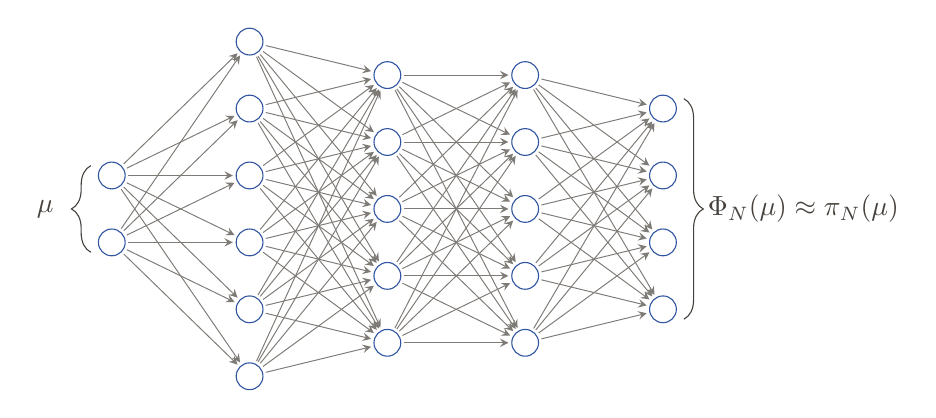
\begin{tikzpicture}

  \layer{input}{\nin}{0}
  \layer{hiddenA}{6}{\hsep}
  \layer{hiddenB}{5}{2*\hsep}
  \layer{hiddenC}{5}{3*\hsep}
  \layer{output}{\nout}{4*\hsep}

  \connect{input}{\nin}{hiddenA}{6}
  \connect{hiddenA}{6}{hiddenB}{5}
  \connect{hiddenB}{5}{hiddenC}{5}
  \connect{hiddenC}{5}{output}{\nout}

  % --- inputs --------------------------------------------------------------
  % the parameter always occupies the first two neurons; for the
  % random-access-in-time variant the time instance enters as a third input
  \draw[brace mirrored] (input-1.north west) -- (input-2.south west)
    node[midway, xshift=-0.72cm, text=DarkGray] {$\mu$};
  \ifnum\variant=2
    \node[left=0.5cm of input-3, text=DarkGray, inner sep=1pt] (t) {$t$};
    \draw[->, >=stealth, draw=DarkGray] (t) -- (input-3.west);
  \fi

  % --- output --------------------------------------------------------------
  \ifnum\variant=1
    \def\outlabel{$\Phi_N(\mu)\approx\pi_N(\mu)$}
  \fi
  \ifnum\variant=2
    \def\outlabel{$\Phi_N(\mu,t)\approx\pi_N(\mu,t)$}
  \fi
  \ifnum\variant=3
    \def\outlabel{$\Phi_N(\mu)\approx\big[\pi_N(\mu,t_1),\ldots,\pi_N(\mu,t_K)\big]$}
  \fi

  \draw[brace] (output-1.north east) -- (output-\nout.south east)
    node[midway, right=0.32cm, text=DarkGray] {\outlabel};

\end{tikzpicture}
\end{document}
"
%   done
%   pdftoppm -png -r 1200 nn_variant1.pdf nn_stationary   % etc., then rename
% 1200 dpi matches the other figures in this directory.

\documentclass[11pt,border=2mm]{standalone}

\usepackage{amsmath}
\usepackage{tikz}
\usetikzlibrary{positioning,calc,decorations.pathreplacing}

\definecolor{pymor_blue}{HTML}{3155a0}
\definecolor{DarkGray}{rgb}{0.274509804,0.254901961,0.235294118}

\providecommand{\variant}{1}

\tikzset{
  neuron/.style={circle, draw=pymor_blue, fill=white, minimum size=0.34cm, inner sep=0pt},
  arrow/.style={->, >=stealth, draw=DarkGray!70, line width=0.35pt, shorten >=1pt, shorten <=1pt},
  brace/.style={decorate, decoration={brace, amplitude=7pt, raise=4pt}, draw=DarkGray},
  brace mirrored/.style={decorate, decoration={brace, amplitude=7pt, mirror, raise=4pt}, draw=DarkGray},
}

\newcommand{\vsep}{0.85}   % vertical distance between neurons
\newcommand{\hsep}{1.75}   % horizontal distance between layers

% #1 layer name, #2 number of neurons, #3 x position -- vertically centred on y=0
\newcommand{\layer}[3]{%
  \foreach \i in {1,...,#2} {%
    \pgfmathsetmacro{\ypos}{-(\i - (#2+1)/2)*\vsep}%
    \node[neuron] (#1-\i) at (#3,\ypos) {};%
  }%
}

% #1 source name, #2 source count, #3 target name, #4 target count
\newcommand{\connect}[4]{%
  \foreach \i in {1,...,#2} {\foreach \j in {1,...,#4} {\draw[arrow] (#1-\i) -- (#3-\j);}}%
}

% number of input and output neurons for the selected variant
\ifnum\variant=2 \def\nin{3}\else\def\nin{2}\fi
\ifnum\variant=3 \def\nout{12}\else\def\nout{4}\fi

\begin{document}
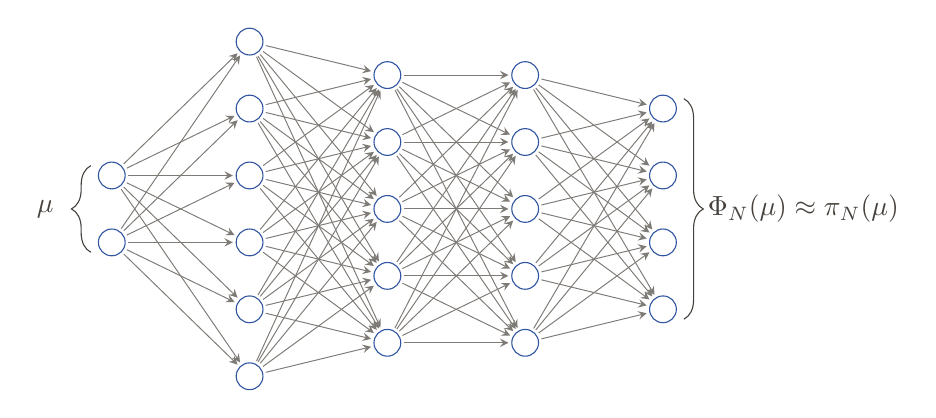
\begin{tikzpicture}

  \layer{input}{\nin}{0}
  \layer{hiddenA}{6}{\hsep}
  \layer{hiddenB}{5}{2*\hsep}
  \layer{hiddenC}{5}{3*\hsep}
  \layer{output}{\nout}{4*\hsep}

  \connect{input}{\nin}{hiddenA}{6}
  \connect{hiddenA}{6}{hiddenB}{5}
  \connect{hiddenB}{5}{hiddenC}{5}
  \connect{hiddenC}{5}{output}{\nout}

  % --- inputs --------------------------------------------------------------
  % the parameter always occupies the first two neurons; for the
  % random-access-in-time variant the time instance enters as a third input
  \draw[brace mirrored] (input-1.north west) -- (input-2.south west)
    node[midway, xshift=-0.72cm, text=DarkGray] {$\mu$};
  \ifnum\variant=2
    \node[left=0.5cm of input-3, text=DarkGray, inner sep=1pt] (t) {$t$};
    \draw[->, >=stealth, draw=DarkGray] (t) -- (input-3.west);
  \fi

  % --- output --------------------------------------------------------------
  \ifnum\variant=1
    \def\outlabel{$\Phi_N(\mu)\approx\pi_N(\mu)$}
  \fi
  \ifnum\variant=2
    \def\outlabel{$\Phi_N(\mu,t)\approx\pi_N(\mu,t)$}
  \fi
  \ifnum\variant=3
    \def\outlabel{$\Phi_N(\mu)\approx\big[\pi_N(\mu,t_1),\ldots,\pi_N(\mu,t_K)\big]$}
  \fi

  \draw[brace] (output-1.north east) -- (output-\nout.south east)
    node[midway, right=0.32cm, text=DarkGray] {\outlabel};

\end{tikzpicture}
\end{document}
"
%   done
%   pdftoppm -png -r 1200 nn_variant1.pdf nn_stationary   % etc., then rename
% 1200 dpi matches the other figures in this directory.

\documentclass[11pt,border=2mm]{standalone}

\usepackage{amsmath}
\usepackage{tikz}
\usetikzlibrary{positioning,calc,decorations.pathreplacing}

\definecolor{pymor_blue}{HTML}{3155a0}
\definecolor{DarkGray}{rgb}{0.274509804,0.254901961,0.235294118}

\providecommand{\variant}{1}

\tikzset{
  neuron/.style={circle, draw=pymor_blue, fill=white, minimum size=0.34cm, inner sep=0pt},
  arrow/.style={->, >=stealth, draw=DarkGray!70, line width=0.35pt, shorten >=1pt, shorten <=1pt},
  brace/.style={decorate, decoration={brace, amplitude=7pt, raise=4pt}, draw=DarkGray},
  brace mirrored/.style={decorate, decoration={brace, amplitude=7pt, mirror, raise=4pt}, draw=DarkGray},
}

\newcommand{\vsep}{0.85}   % vertical distance between neurons
\newcommand{\hsep}{1.75}   % horizontal distance between layers

% #1 layer name, #2 number of neurons, #3 x position -- vertically centred on y=0
\newcommand{\layer}[3]{%
  \foreach \i in {1,...,#2} {%
    \pgfmathsetmacro{\ypos}{-(\i - (#2+1)/2)*\vsep}%
    \node[neuron] (#1-\i) at (#3,\ypos) {};%
  }%
}

% #1 source name, #2 source count, #3 target name, #4 target count
\newcommand{\connect}[4]{%
  \foreach \i in {1,...,#2} {\foreach \j in {1,...,#4} {\draw[arrow] (#1-\i) -- (#3-\j);}}%
}

% number of input and output neurons for the selected variant
\ifnum\variant=2 \def\nin{3}\else\def\nin{2}\fi
\ifnum\variant=3 \def\nout{12}\else\def\nout{4}\fi

\begin{document}
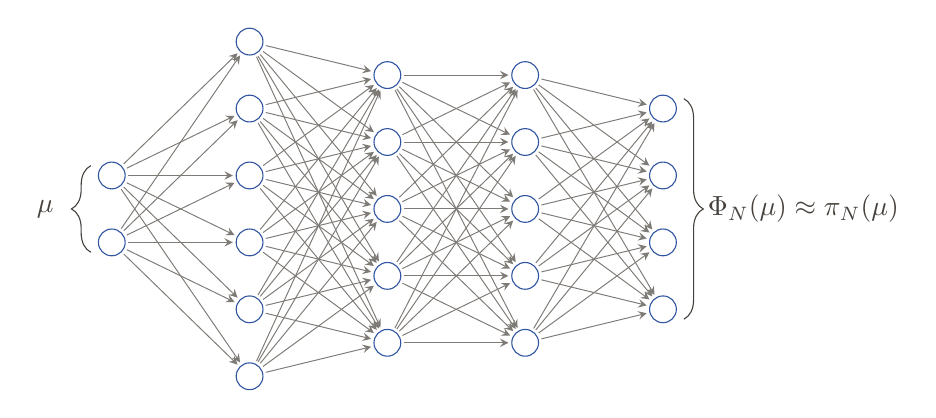
\begin{tikzpicture}

  \layer{input}{\nin}{0}
  \layer{hiddenA}{6}{\hsep}
  \layer{hiddenB}{5}{2*\hsep}
  \layer{hiddenC}{5}{3*\hsep}
  \layer{output}{\nout}{4*\hsep}

  \connect{input}{\nin}{hiddenA}{6}
  \connect{hiddenA}{6}{hiddenB}{5}
  \connect{hiddenB}{5}{hiddenC}{5}
  \connect{hiddenC}{5}{output}{\nout}

  % --- inputs --------------------------------------------------------------
  % the parameter always occupies the first two neurons; for the
  % random-access-in-time variant the time instance enters as a third input
  \draw[brace mirrored] (input-1.north west) -- (input-2.south west)
    node[midway, xshift=-0.72cm, text=DarkGray] {$\mu$};
  \ifnum\variant=2
    \node[left=0.5cm of input-3, text=DarkGray, inner sep=1pt] (t) {$t$};
    \draw[->, >=stealth, draw=DarkGray] (t) -- (input-3.west);
  \fi

  % --- output --------------------------------------------------------------
  \ifnum\variant=1
    \def\outlabel{$\Phi_N(\mu)\approx\pi_N(\mu)$}
  \fi
  \ifnum\variant=2
    \def\outlabel{$\Phi_N(\mu,t)\approx\pi_N(\mu,t)$}
  \fi
  \ifnum\variant=3
    \def\outlabel{$\Phi_N(\mu)\approx\big[\pi_N(\mu,t_1),\ldots,\pi_N(\mu,t_K)\big]$}
  \fi

  \draw[brace] (output-1.north east) -- (output-\nout.south east)
    node[midway, right=0.32cm, text=DarkGray] {\outlabel};

\end{tikzpicture}
\end{document}
